\documentclass[64pt]{beamer}

\usetheme{mpiisimple}

\usepackage{soul}
\usepackage{pdfcomment}
\usepackage[utf8]{inputenc}
%\usepackage{times}
%\usepackage{epsfig}
\usepackage{graphicx}
\usepackage{amsmath,amsfonts,amssymb,amsthm}
\usepackage{xspace}
\usepackage{xcolor}
\usepackage{tabularx}
%\usepackage{pifont}
%\usepackage{caption}
%\captionsetup{justification=centering,font=large}
%\usepackage{subcaption}
%\usepackage{algorithm}
%\usepackage[noend]{algorithmic}
\usepackage{nicefrac}
%\usepackage{pgfplots}
%\usepackage{pgfplotstable}
%\usepackage{bbm}
%\usepackage{multirow}
\usepackage[skins]{tcolorbox}
%\usepackage{transparent}
\usepackage{tikz}
%\usepackage{tikz-3dplot}
%\usetikzlibrary{matrix}
\usetikzlibrary{calc}
\usetikzlibrary{fadings}
%\usetikzlibrary{intersections}
\usetikzlibrary{arrows.new}
%\usetikzlibrary{backgrounds}
%\usepgfplotslibrary{fillbetween}
%\usetikzlibrary{intersections}
\tikzset{arrow/.style={-latex new,arrow head=0.25cm}}
\newcommand*\circled[1]{\tikz[baseline=(char.base)]{
		\node[shape=circle,draw=MPIIorange,fill=MPIIorange,inner sep=2pt] (char) {\color{MPIIwhite}#1};}}
	
\definecolor{colorbrewer1}{RGB}{228,26,28}
\definecolor{colorbrewer2}{RGB}{55,126,184}
\definecolor{colorbrewer3}{RGB}{77,175,74}
\definecolor{colorbrewer4}{RGB}{152,78,163}
\definecolor{colorbrewer5}{RGB}{255,127,0}
\definecolor{colorbrewer6}{RGB}{255,255,51}
\definecolor{colorbrewer7}{RGB}{166,86,40}
\definecolor{colorbrewer8}{RGB}{247,129,191}
\definecolor{colorbrewer9}{RGB}{153,153,153}

\DeclareMathOperator*{\argmax}{argmax~}
\DeclareMathOperator*{\argmin}{argmin~}
\DeclareMathOperator{\sign}{sign}
\DeclareMathOperator*{\ntimes}{\!\times\!}
\newcommand{\Id}{\mathbbm{1}}
\DeclareRobustCommand{\RTE}{%
	\ifmmode
	\text{RErr}
	\else
	RErr\xspace
	\fi
}

\makeatletter
\DeclareRobustCommand\onedot{\futurelet\@let@token\@onedot}
\def\@onedot{\ifx\@let@token.\else.\null\fi\xspace}
\def\eg{e.g\onedot} \def\Eg{E.g\onedot}
\def\ie{i.e\onedot} \def\Ie{I.e\onedot}
\def\cf{cf\onedot} \def\Cf{Cf\onedot}
\def\etc{etc\onedot} \def\vs{vs\onedot}
\def\st{s.t\onedot}
\def\wrt{wrt\onedot}
\def\dof{d.o.f\onedot}
\def\etal{et~al\onedot} \def\iid{i.i.d\onedot}
\def\Fig{Fig\onedot} \def\Eqn{Eqn\onedot} \def\Sec{Sec\onedot} \def\Alg{Alg\onedot}
\makeatother

\author{David Stutz}
\title[Confidence-Calibrated Adversarial Training]{Confidence Calibration of Adversarial Training}

\begin{document}
	\setbeamertemplate{footline}{
		\begin{textblock*}{\paperwidth}(4mm,88mm)
			\begin{minipage}{40mm}
				
\includegraphics[scale=0.045]{mpilogo-inf-wide}
			\end{minipage}
			\begin{minipage}{27.5mm}
				
\includegraphics[scale=0.15]{UT_WBMW_Rot_RGB}
			\end{minipage}
			%\hfill
			\begin{minipage}{55mm}
				\raggedright\tiny{\textcolor{MPIIblue}{\insertshorttitle \ {\color{MPIIgray}--} \insertauthor}}
			\end{minipage}
			\vspace*{4mm}
		\end{textblock*}
	}
	
	\begingroup
	\setbeamertemplate{footline}{}
	\begin{frame}[plain,noframenumbering]
		\begin{center}  
			{\Huge\bfseries Confidence-Calibrated\\[10px] Adversarial Training}
			\vskip 0.5em
			
			{\LARGE Generalizing to Unseen Attacks}
			\vskip 1em
			
			{\Large David Stutz, Matthias Hein, Bernt Schiele}
			\vskip 0.5em
			
			%{\large\color{MPIIdarkergray} with Bernt Schiele, Matthias Hein}
			%\vskip 1em
			
			\begin{minipage}[t]{4.75cm}
				\vspace*{0px}
				\centering
				\begin{tikzpicture}
				\node at (0,0){
\includegraphics[height=1.3cm]{mpilogo-inf-narrow.eps}};
				\end{tikzpicture}
			\end{minipage}
			\hspace*{0.25cm}
			\begin{minipage}[t]{4.75cm}
				\vspace*{0px}
				\centering
				\begin{tikzpicture}
				\node at (0,0){
\includegraphics[height=1.3cm]{UT_WBMW_Rot_RGB.eps}};
				\end{tikzpicture}
			\end{minipage}
		\end{center}
	\end{frame}
	\endgroup
	
	\begin{frame}[t]{\bfseries \textit{2-Minute} Overview}
		\Large
		
		Problem: Robustness to \emph{various} adversarial examples.
		\vskip 0.25cm
		
		Adversarial training on $L_\infty$ adversarial examples:
		\vskip -0.25cm 
		%\vskip -0.25cm
		\begin{minipage}[t]{0.7\textwidth}
			\vspace*{0px}
			\hfill
			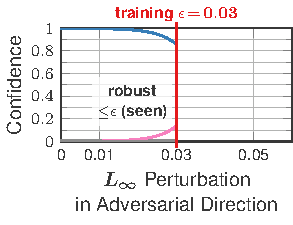
\includegraphics[width=7cm]{fig/introduction/advtrain_1_adversarial_seen}
		\end{minipage}
		\hfill
		\begin{minipage}[t]{0.28\textwidth}
			\vspace*{15px}
			
			\begin{tcolorbox}[
				left=0pt,
				right=0pt,
				top=0pt,
				bottom=0pt,
				colback=gray!12!white,
				colframe=gray!12!white,
				width=1\textwidth, 
				enlarge left by=0mm,
				boxsep=5pt,
				arc=0pt,outer arc=0pt,
				%coltitle=black,
				%title=Training,
				boxrule=1pt,
				]
				\large\color{MPIIblack}
				SVHN:\\
				\textcolor{colorbrewer2}{{\rule[4pt]{10pt}{2pt} Correct}}\\ \textcolor{colorbrewer8}{{\rule[4pt]{10pt}{2pt} Adversarial}}
			\end{tcolorbox}
		\end{minipage}
	\end{frame}

	\begin{frame}[t]{\bfseries \textit{2-Minute} Overview}
		\Large
		
		Problem: Robustness to \emph{various} adversarial examples.
		\vskip 0.25cm
		
		Adversarial training on $L_\infty$ adversarial examples:
		\vskip -0.25cm 
		%\vskip -0.25cm
		\begin{minipage}[t]{0.7\textwidth}
			\vspace*{0px}
			\hfill
			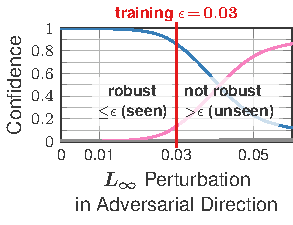
\includegraphics[width=7cm]{fig/introduction/advtrain_1_adversarial_unseen}
		\end{minipage}
		\hfill
		\begin{minipage}[t]{0.28\textwidth}
			\vspace*{15px}
			
			\begin{tcolorbox}[
				left=0pt,
				right=0pt,
				top=0pt,
				bottom=0pt,
				colback=gray!12!white,
				colframe=gray!12!white,
				width=1\textwidth, 
				enlarge left by=0mm,
				boxsep=5pt,
				arc=0pt,outer arc=0pt,
				%coltitle=black,
				%title=Training,
				boxrule=1pt,
				]
				\large\color{MPIIblack}
				SVHN:\\
				\textcolor{colorbrewer2}{{\rule[4pt]{10pt}{2pt} Correct}}\\ \textcolor{colorbrewer8}{{\rule[4pt]{10pt}{2pt} Adversarial}}
			\end{tcolorbox}
		\end{minipage}
	\end{frame}

	\begin{frame}[t]{\bfseries \textit{2-Minute} Overview}
		\Large
		
		Problem: Robustness to various adversarial examples.
		\vskip 0.25cm
		
		Adversarial training on {\color{MPIIred}$L_\infty$} adversarial examples:
		
		%\vskip -0.25cm
		\begin{minipage}[t]{0.7\textwidth}
			\vspace*{0px}
			\hfill
			\only<1>{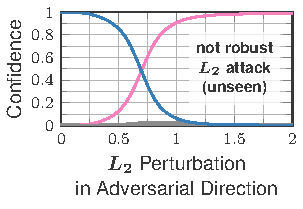
\includegraphics[width=7cm]{fig/introduction/advtrain_3_l2_adversarial}}
		\end{minipage}
		\hfill
		\begin{minipage}[t]{0.28\textwidth}
			\vspace*{4px}
			
			\begin{tcolorbox}[
				left=0pt,
				right=0pt,
				top=0pt,
				bottom=0pt,
				colback=gray!12!white,
				colframe=gray!12!white,
				width=1\textwidth, 
				enlarge left by=0mm,
				boxsep=5pt,
				arc=0pt,outer arc=0pt,
				%coltitle=black,
				%title=Training,
				boxrule=1pt,
				]
				\large\color{MPIIblack}
				SVHN:\\
				\textcolor{colorbrewer2}{{\rule[4pt]{10pt}{2pt} Correct}}\\ \textcolor{colorbrewer8}{{\rule[4pt]{10pt}{2pt} Adversarial}}
			\end{tcolorbox}
		\end{minipage}
	\end{frame}

%	\begin{frame}[t]{\bfseries \textit{2-Minute} Overview}
%		\large
%		
%		Adversarial training:
%		
%		\vskip -0.1cm
%		\begin{minipage}[t]{0.7\textwidth}
%			\vspace*{0px}
%			\hfill
%			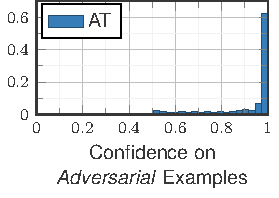
\includegraphics[width=6.25cm]{fig/histograms/succ_advtrain}
%		\end{minipage}
%		\begin{minipage}[t]{0.28\textwidth}
%			\vspace*{0px}
%		\end{minipage}
%	\end{frame}

	\begin{frame}[t]{\bfseries \textit{2-Minute} Overview}
		\Large
		
		\begin{tcolorbox}[
			enhanced,
			boxsep=0pt,
			left=5pt,
			right=5pt,
			top=2pt,
			toptitle=4pt,
			bottomtitle=2pt,
			bottom=2pt,
			colback=white,
			colframe=white,
			width=1\textwidth, 
			enlarge left by=0mm,
			arc=0pt,outer arc=0pt,
			%coltitle=black,
			%title=Training,
			boxrule=1pt,
			title=Summary of adversarial training:,
			coltitle=MPIIblack,
			colbacktitle=white,
			titlerule style=white,
			]
			
			%\vspace*{-4px}
			\centering
			\begin{minipage}[t]{0.45\textwidth}
				\vspace*{0px}
				\hfill
				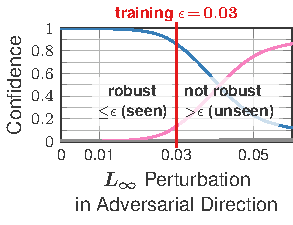
\includegraphics[width=5cm]{fig/introduction/advtrain_1_adversarial_unseen}
			\end{minipage}
			\begin{minipage}[t]{0.45\textwidth}
				\vspace*{7px}
				\hfill
				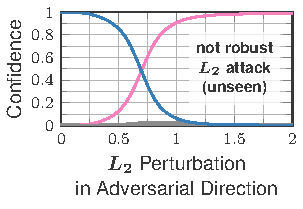
\includegraphics[width=5.15cm]{fig/introduction/advtrain_3_l2_adversarial}
			\end{minipage}
%			\begin{minipage}[t]{0.3\textwidth}
%				\vspace*{10px}
%				\centering
%				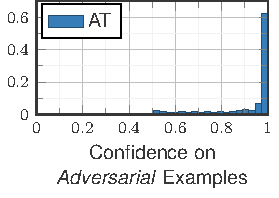
\includegraphics[width=3.5cm]{fig/histograms/succ_advtrain}
%				\hfill
%			\end{minipage}
			\vspace*{-2px}
		\end{tcolorbox}
		\vspace*{-0.5cm}
		
		\begin{itemize}
			\item High-confidence on adversarial examples (${\leq}\epsilon$).
			\item \emph{No} generalization to larger/other $L_p$ perturbations.
			\item Behavior not meaningful for arbitrarily large $\epsilon$.
		\end{itemize}
	\end{frame}

	\begin{frame}[t]{\bfseries \textit{2-Minute} Overview}
		\Large
		
	    Confidence-calibrated adversarial training ($L_\infty$ \emph{only}):
		
		\vskip -0.25cm
		\begin{minipage}[t]{0.7\textwidth}
			\vspace*{0px}
			\hfill
			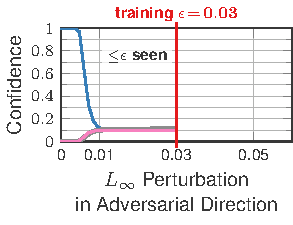
\includegraphics[width=7cm]{fig/introduction/ours10_1_adversarial_seen}
		\end{minipage}
		\hfill
		\begin{minipage}[t]{0.28\textwidth}
			\vspace*{15px}
			
			\begin{tcolorbox}[
				left=0pt,
				right=0pt,
				top=0pt,
				bottom=0pt,
				colback=gray!12!white,
				colframe=gray!12!white,
				width=1\textwidth, 
				enlarge left by=0mm,
				boxsep=5pt,
				arc=0pt,outer arc=0pt,
				%coltitle=black,
				%title=Training,
				boxrule=1pt,
				]
				\large\color{MPIIblack}
				SVHN:\\
				\textcolor{colorbrewer2}{{\rule[4pt]{10pt}{2pt} Correct}}\\ \textcolor{colorbrewer8}{{\rule[4pt]{10pt}{2pt} Adversarial}}
			\end{tcolorbox}
		\end{minipage}
	\end{frame}

	\begin{frame}[t]{\bfseries \textit{2-Minute} Overview}
		\Large
		
		Confidence-calibrated adversarial training ($L_\infty$ \emph{only}):
		
		\vskip -0.25cm
		\begin{minipage}[t]{0.7\textwidth}
			\vspace*{0px}
			\hfill
			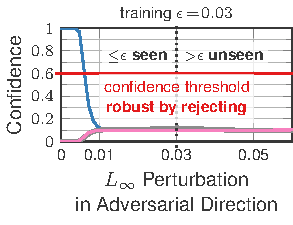
\includegraphics[width=7cm]{fig/introduction/ours10_1_adversarial_unseen_annotated}
		\end{minipage}
		\hfill
		\begin{minipage}[t]{0.28\textwidth}
			\vspace*{15px}
			
			\begin{tcolorbox}[
				left=0pt,
				right=0pt,
				top=0pt,
				bottom=0pt,
				colback=gray!12!white,
				colframe=gray!12!white,
				width=1\textwidth, 
				enlarge left by=0mm,
				boxsep=5pt,
				arc=0pt,outer arc=0pt,
				%coltitle=black,
				%title=Training,
				boxrule=1pt,
				]
				\large\color{MPIIblack}
				SVHN:\\
				\textcolor{colorbrewer2}{{\rule[4pt]{10pt}{2pt} Correct}}\\ \textcolor{colorbrewer8}{{\rule[4pt]{10pt}{2pt} Adversarial}}
			\end{tcolorbox}
		\end{minipage}
	\end{frame}

	\begin{frame}[t]{\bfseries \textit{2-Minute} Overview}
		\Large
		
	    Confidence-calibrated adversarial training ($L_\infty$ \emph{only}):
		
		\vskip -0.25cm
		\begin{minipage}[t]{0.7\textwidth}
			\vspace*{0px}
			\hfill
			%\only<1>{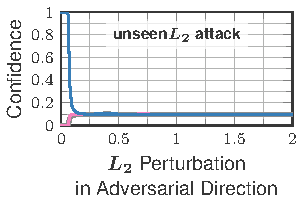
\includegraphics[width=6.5cm]{fig/introduction/ours10_3_l2_adversarial}}
			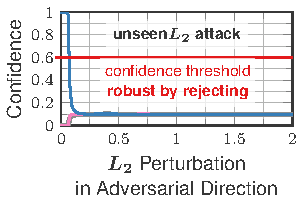
\includegraphics[width=6.5cm]{fig/introduction/ours10_3_l2_adversarial_annotated}
		\end{minipage}
		\hfill
		\begin{minipage}[t]{0.28\textwidth}
			\vspace*{4px}
			
			\begin{tcolorbox}[
				left=0pt,
				right=0pt,
				top=0pt,
				bottom=0pt,
				colback=gray!12!white,
				colframe=gray!12!white,
				width=1\textwidth, 
				enlarge left by=0mm,
				boxsep=5pt,
				arc=0pt,outer arc=0pt,
				%coltitle=black,
				%title=Training,
				boxrule=1pt,
				]
				\large
				SVHN:\\
				\textcolor{colorbrewer2}{{\rule[4pt]{10pt}{2pt} Correct}}\\ \textcolor{colorbrewer8}{{\rule[4pt]{10pt}{2pt} Adversarial}}
			\end{tcolorbox}
		\end{minipage}
	\end{frame}

%	\begin{frame}[t]{\bfseries \textit{2-Minute} Overview}
%		\large
%		
%	    Confidence-calibrated adversarial training:
%		
%		\vskip -0.1cm
%		\begin{minipage}[t]{0.7\textwidth}
%			\vspace*{0px}
%			\hfill
%			\only<1>{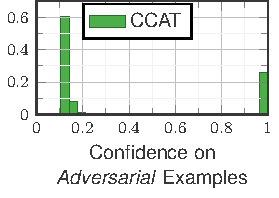
\includegraphics[width=6.25cm]{fig/histograms/succ_ours10}}
%			\only<2>{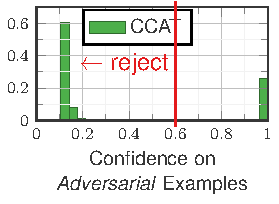
\includegraphics[width=6.25cm]{fig/histograms/succ_ours10_annotated}}
%		\end{minipage}
%		\begin{minipage}[t]{0.28\textwidth}
%			\vspace*{0px}
%		\end{minipage}
%	\end{frame}

%	\begin{frame}[t]{\bfseries \textit{2-Minute} Overview}
%		\large
%		
%		\begin{tcolorbox}[
%			enhanced,
%			boxsep=0pt,
%			left=5pt,
%			right=5pt,
%			top=2pt,
%			toptitle=4pt,
%			bottomtitle=2pt,
%			bottom=2pt,
%			colback=gray!12!white,
%			colframe=gray!12!white,
%			width=1\textwidth, 
%			enlarge left by=0mm,
%			arc=0pt,outer arc=0pt,
%			%coltitle=black,
%			%title=Training,
%			boxrule=1pt,
%			title=Confidence-calibrated adversarial training (CCAT):,
%			coltitle=MPIIblack,
%			colbacktitle=gray!12!white,
%			titlerule style=white,%gray!25!white,
%			]
%			
%			%\vspace*{-4px}
%			\centering
%			\begin{minipage}[t]{0.35\textwidth}
%				\vspace*{0px}
%				\hfill
%				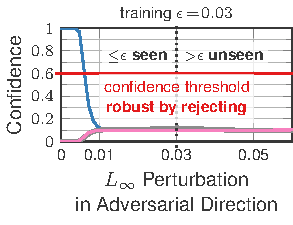
\includegraphics[width=3.75cm]{fig/introduction/ours10_1_adversarial_unseen_annotated}
%			\end{minipage}
%			\begin{minipage}[t]{0.35\textwidth}
%				\vspace*{6px}
%				\hfill
%				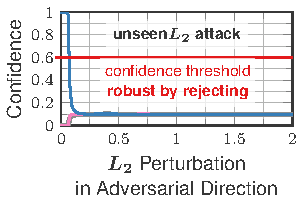
\includegraphics[width=3.8cm]{fig/introduction/ours10_3_l2_adversarial_annotated}
%			\end{minipage}
%%			\begin{minipage}[t]{0.3\textwidth}
%%				\vspace*{9px}
%%				\centering
%%				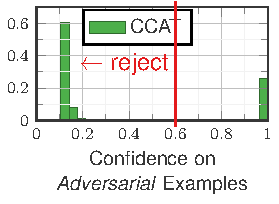
\includegraphics[width=3.5cm]{fig/histograms/succ_ours10_annotated}
%%				\hfill
%%			\end{minipage}
%			\vspace*{-2px}
%		\end{tcolorbox}
%	
%		\begin{itemize}
%			\item Low-confidence on adversarial examples \emph{and beyond}.
%			\item {\bfseries \color{MPIIred} Robustness to previously \emph{unseen} perturbations} by confidence thresholding.
%		\end{itemize}
%	\end{frame}

%	\begin{frame}[t]{\bfseries \textit{2-Minute} Overview}
%		\large
%		
%		\vskip -0.25cm
%		\begin{tcolorbox}[
%			enhanced,
%			boxsep=0pt,
%			left=5pt,
%			right=5pt,
%			top=0pt,
%			toptitle=4pt,
%			bottomtitle=2pt,
%			bottom=0pt,
%			colback=white,
%			colframe=gray!25!white,
%			width=1\textwidth, 
%			enlarge left by=0mm,
%			arc=0pt,outer arc=0pt,
%			%coltitle=black,
%			%title=Training,
%			boxrule=1pt,
%			title=Adversarial training (AT):,
%			coltitle=MPIIblack,
%			colbacktitle=white,
%			titlerule style=gray!25!white,
%			]
%			
%			%\vspace*{-4px}
%			\centering
%			\begin{minipage}[t]{0.35\textwidth}
%				\vspace*{0px}
%				\centering
%				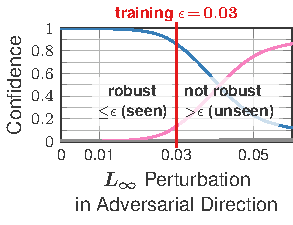
\includegraphics[width=3.75cm]{fig/introduction/advtrain_1_adversarial_unseen}
%			\end{minipage}
%			\begin{minipage}[t]{0.35\textwidth}
%				\vspace*{5px}
%				\centering
%				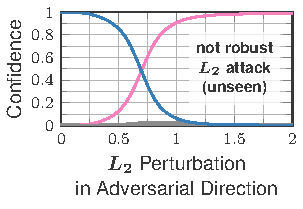
\includegraphics[width=3.8cm]{fig/introduction/advtrain_3_l2_adversarial}
%			\end{minipage}
%%			\begin{minipage}[t]{0.3\textwidth}
%%				\vspace*{9px}
%%				\centering
%%				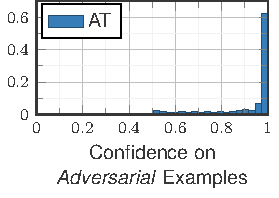
\includegraphics[width=3.5cm]{fig/histograms/succ_advtrain}
%%				\hfill
%%			\end{minipage}
%			\vspace*{-2px}
%		\end{tcolorbox}
%		\vspace*{-4px}
%		
%		\begin{tcolorbox}[
%			enhanced,
%			boxsep=0pt,
%			left=5pt,
%			right=5pt,
%			top=0pt,
%			toptitle=4pt,
%			bottomtitle=2pt,
%			bottom=0pt,
%			colback=gray!12!white,
%			colframe=gray!12!white,
%			width=1\textwidth, 
%			enlarge left by=0mm,
%			arc=0pt,outer arc=0pt,
%			%coltitle=black,
%			%title=Training,
%			boxrule=1pt,
%			title=Confidence-calibrated adversarial training (CCAT):,
%			coltitle=MPIIblack,
%			colbacktitle=gray!12!white,
%			titlerule style=white,%gray!25!white,
%			]
%			
%			%\vspace*{-4px}
%			\centering
%			\begin{minipage}[t]{0.35\textwidth}
%				\vspace*{0px}
%				\centering
%				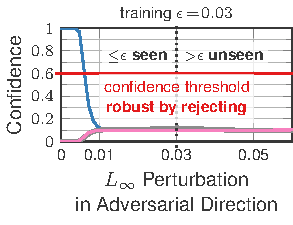
\includegraphics[width=3.75cm]{fig/introduction/ours10_1_adversarial_unseen_annotated}
%			\end{minipage}
%			\begin{minipage}[t]{0.35\textwidth}
%				\vspace*{6px}
%				\centering
%				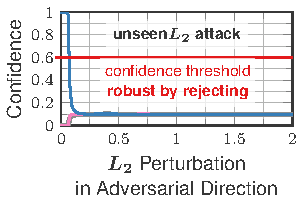
\includegraphics[width=3.8cm]{fig/introduction/ours10_3_l2_adversarial_annotated}
%			\end{minipage}
%%			\begin{minipage}[t]{0.3\textwidth}
%%				\vspace*{8px}
%%				\centering
%%				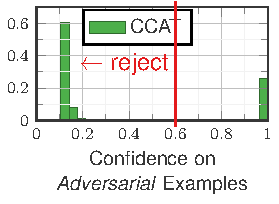
\includegraphics[width=3.5cm]{fig/histograms/succ_ours10_annotated}
%%				\hfill
%%			\end{minipage}
%			\vspace*{-2px}
%		\end{tcolorbox}
%	\end{frame}

	\begin{frame}[t]{\bfseries \textit{2-Minute} Overview}
		\Large
		
		\vspace*{-0.15cm}
		\begin{tcolorbox}[
			enhanced,
			boxsep=0pt,
			left=5pt,
			right=5pt,
			top=0pt,
			toptitle=4pt,
			bottomtitle=2pt,
			bottom=0pt,
			colback=white,
			colframe=white,
			width=1\textwidth, 
			enlarge left by=0mm,
			arc=0pt,outer arc=0pt,
			%coltitle=black,
			%title=Training,
			boxrule=1pt,
			title=Adversarial training:,
			coltitle=MPIIblack,
			colbacktitle=white,
			titlerule style=white,
			]
			
			%\vspace*{-4px}
			\begin{minipage}[t]{0.375\textwidth}
				\vspace*{0px}
				%\hfill
				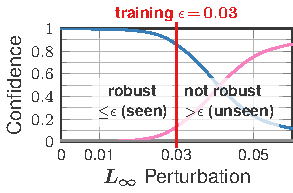
\includegraphics[width=4.25cm]{fig/introduction/advtrain_1_adversarial_unseen_narrow}
			\end{minipage}
			\begin{minipage}[t]{0.625\textwidth}
				\vspace*{10px}
				\normalsize
				{\color{MPIIblue}\footnotesize $\blacktriangleright$} {\color{MPIIblack} High-confidence on adversarial examples.}\\[2px]
				{\color{MPIIblue}\footnotesize $\blacktriangleright$} {\color{MPIIblack} No robustness to \emph{unseen} perturbations.}
			\end{minipage}
			\vspace*{-2px}
		\end{tcolorbox}
		\vspace*{-0.1cm}
		
		\begin{tcolorbox}[
			enhanced,
			boxsep=0pt,
			left=5pt,
			right=5pt,
			top=0pt,
			toptitle=4pt,
			bottomtitle=2pt,
			bottom=0pt,
			colback=gray!12!white,
			colframe=gray!12!white,
			width=1\textwidth, 
			enlarge left by=0mm,
			arc=0pt,outer arc=0pt,
			%coltitle=black,
			%title=Training,
			boxrule=1pt,
			title=Confidence-calibrated adversarial training:,
			coltitle=MPIIblack,
			colbacktitle=gray!12!white,
			titlerule style=white,%gray!25!white,
			collower=MPIIblack,
			]
			%\vspace*{-4px}
			\begin{minipage}[t]{0.375\textwidth}
				\vspace*{0px}
				%\hfill
				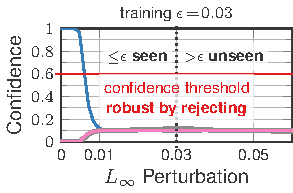
\includegraphics[width=4.25cm]{fig/introduction/ours10_1_adversarial_unseen_annotated_narrow}
			\end{minipage}
			\begin{minipage}[t]{0.625\textwidth}
				\vspace*{10px}
				\normalsize
				{\color{MPIIblue}\footnotesize $\blacktriangleright$} {\color{MPIIblack} Low-confidence on adversarial examples.}\\[2px]
				{\color{MPIIblue}\footnotesize $\blacktriangleright$} {\bfseries \color{MPIIred} Robustness to \emph{unseen} perturbations}\\
				\hspace*{12px}{\color{MPIIblack}by confidence thresholding.}
			\end{minipage}
			\vspace*{-2px}
		\end{tcolorbox}
	\end{frame}

	\begin{frame}[t]{\bfseries Interested?}
		\Large
		
		\begin{tcolorbox}[
			enhanced,
			boxsep=4pt,
			left=0pt,
			right=0pt,
			top=2pt,
			toptitle=0pt,
			bottomtitle=2pt,
			bottom=0pt,
			colback=gray!12!white,
			colframe=gray!12!white,
			width=1\textwidth, 
			enlarge left by=0mm,
			arc=0pt,outer arc=0pt,
			%coltitle=black,
			%title=Training,
			boxrule=1pt,
			title=\bfseries More details:,
			coltitle=MPIIblack,
			colbacktitle=gray!12!white,
			titlerule style=white,%gray!25!white,
			collower=MPIIblack,
			]
			\color{MPIIblack}
			Paper \& code: \href{http://davidstutz.de/ccat}{\texttt{davidstutz.de/ccat}}\\
			Contact: \texttt{david.stutz@mpi-inf.mpg.de}
		\end{tcolorbox}
	\end{frame}
    
	\begin{frame}[t]{\bfseries Interested?}
		\Large
		
		\begin{tcolorbox}[
			enhanced,
			boxsep=4pt,
			left=0pt,
			right=0pt,
			top=2pt,
			toptitle=0pt,
			bottomtitle=2pt,
			bottom=0pt,
			colback=gray!12!white,
			colframe=gray!12!white,
			width=1\textwidth, 
			enlarge left by=0mm,
			arc=0pt,outer arc=0pt,
			%coltitle=black,
			%title=Training,
			boxrule=1pt,
			title=\bfseries More details:,
			coltitle=MPIIblack,
			colbacktitle=gray!12!white,
			titlerule style=white,%gray!25!white,
			collower=MPIIblack,
			]
			\color{MPIIblack}
			Paper \& code: \href{http://davidstutz.de/ccat}{\texttt{davidstutz.de/ccat}}\\
			Contact: \texttt{david.stutz@mpi-inf.mpg.de}
		\end{tcolorbox}
		\vskip 0.25cm
		
		\textbf{Outline:}
		\vspace*{0.35cm}
		
		\hspace*{0.25cm}\begin{minipage}{\textwidth}
			\begin{enumerate}
				\item Problems of adversarial training
				\item \textit{Confidence-calibrated adversarial training}
				\item Confidence-thresholded robust test error
				\item Results on SVHN and CIFAR10
			\end{enumerate}
		\end{minipage}
	\end{frame}
    
    \begin{frame}[t]{\bfseries Problems of Adversarial Training}
    	\Large
    	
    	Min-max formulation:
    	\begin{align}
	    	\min_w \mathbb{E}_{p(x, y)} \left[\max_{{\color{MPIIred}\boldsymbol{\|\delta\|_\infty \leq \epsilon}}} \mathcal{L}(f(x + \delta; w), y)\right].\notag
    	\end{align}
    	\begin{tikzpicture}[overlay]
	    	\node[MPIIblue] (text1) at (8.4, 2.35) {classifier};
	    	\draw[arrow,MPIIblue] (text1)[out=180,in=75] to (6.6,1.75);
	    	\node[MPIIblue] (text2) at (5, 0.25) {minimizing cross-entropy yields high-confidence};
	    	\draw[arrow,MPIIblue] (text2)[out=30,in=260] to (6,1.2);
    	\end{tikzpicture}
    \end{frame}

	\begin{frame}[t]{\bfseries Problems of Adversarial Training}
		\Large
		
		Min-max formulation:
		\begin{align}
		\min_w \mathbb{E}_{p(x, y)} \left[\max_{{\color{MPIIred}\boldsymbol{\|\delta\|_\infty \leq \epsilon}}} \mathcal{L}(f(x + \delta; w), y)\right].\notag
		\end{align}
		\begin{tikzpicture}[overlay]
			\node[transparent,MPIIblue] (text1) at (8.4, 2.35) {classifier};
			\draw[transparent,arrow,MPIIblue] (text1)[out=180,in=75] to (6.6,1.75);
			\node[transparent,MPIIblue] (text2) at (5, 0.25) {minimizing cross-entropy yields high-confidence};
			\draw[transparent,arrow,MPIIblue] (text2)[out=30,in=260] to (6,1.2);
		\end{tikzpicture}
		
		\vspace*{-1.25cm}
		\begin{center}
			\centering
			\begin{minipage}[t]{0.4\textwidth}
				\vspace*{0px}
				\hfill
				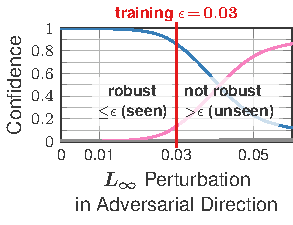
\includegraphics[width=4.75cm]{fig/introduction/advtrain_1_adversarial_unseen}
			\end{minipage}
			\begin{minipage}[t]{0.4\textwidth}
				\vspace*{7px}
				\hfill
				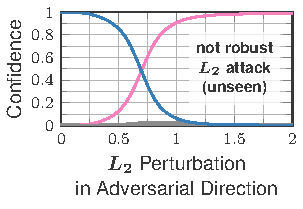
\includegraphics[width=4.9cm]{fig/introduction/advtrain_3_l2_adversarial}
			\end{minipage}
		\end{center}
		\vspace*{-0.5cm}
		\begin{itemize}
			\item Robustness does \emph{not} generalize to unseen attacks.
		\end{itemize}
	\end{frame}
    
%    \begin{frame}[t]{\bfseries Extrapolating High-Confidence Predictions}
%        \Large
%        \vspace*{-0.5cm}
%        \begin{center}
%            \begin{tikzpicture}
%                \node at (0,0){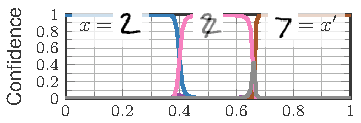
\includegraphics[width=11cm]{fig/interpolation/advtrain_0_interpolation}};
%            \end{tikzpicture}
%        \end{center}
%    \end{frame}
    
    \begin{frame}[t]{\bfseries Confidence-Calibrated Adversarial Training}
        \Large
        \circled{1} Transition to uniform distribution on adversarial examples within the $\epsilon$-ball:
	    \vspace*{-0.5cm}
        \begin{center}
            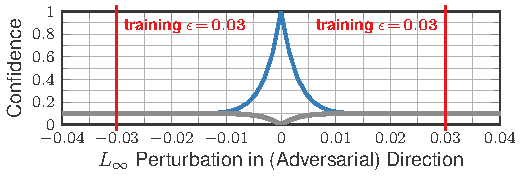
\includegraphics[width=12cm]{fig/transition/confidences_full}
        \end{center}
	    \vskip -0.5cm
	    \begin{itemize}
	    	\item Low-confidence extrapolated beyond $\epsilon$-ball.
	    \end{itemize}
    \end{frame}

%	\begin{frame}[t]{\bfseries Confidence-Calibrated Adversarial Training}
%		\Large
%		\circled{2} Reject (adversarial) examples with low-confidence by confidence-thresholding:
%		\vspace*{0.25cm}
%		\begin{center}
%			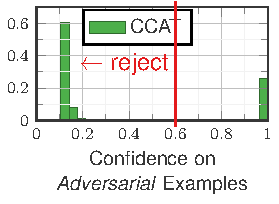
\includegraphics[width=7cm]{fig/histograms/succ_ours10_annotated}
%		\end{center}
%		\vskip -0.5cm
%		\begin{itemize}
%			\item Idea: adversarial examples receive low-confidence.
%		\end{itemize}
%	\end{frame}

%	\begin{frame}[t]{\bfseries Confidence-Calibrated Adversarial Training}
%		\Large
%		\circled{1} Transition to \textbf{low confidence on adversarial examples} within the $\epsilon$-ball.
%		\vskip 0.25em
%		
%		\circled{2} \textbf{Reject low-confidence (adversarial) examples} via {\color{MPIIred}confidence-thresholding}:
%		\vspace*{-0.4cm}
%		
%		\hspace*{-0.25cm}
%		\begin{minipage}[t]{0.49\textwidth}
%			\vspace*{0px}
%			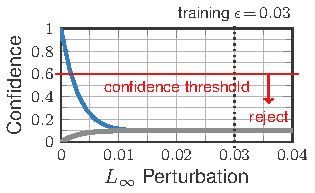
\includegraphics[height=4cm]{fig/transition/confidences_half_annotated}
%		\end{minipage}
%		\hspace*{0.25cm}
%		\begin{minipage}[t]{0.45\textwidth}
%			\vspace*{0.45cm}
%			\hphantom{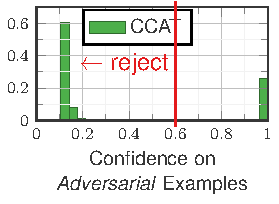
\includegraphics[height=4cm]{fig/histograms/succ_ours10_annotated}}
%		\end{minipage}
%		\hfill
%	\end{frame}

	\begin{frame}[t]{\bfseries Confidence-Calibrated Adversarial Training}
		\Large
		\circled{1} Transition to \textbf{low confidence on adversarial examples} within the $\epsilon$-ball.
		\vskip 0.25em
		
		\circled{2} \textbf{Reject low-confidence (adversarial) examples} via {\color{MPIIred}confidence-thresholding}:
		\vspace*{-0.4cm}
		
		\hspace*{-0.25cm}
		\begin{minipage}[t]{0.49\textwidth}
			\vspace*{0px}
			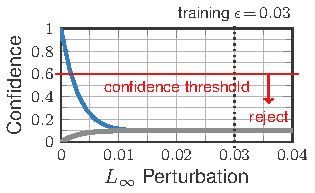
\includegraphics[height=4cm]{fig/transition/confidences_half_annotated}
		\end{minipage}
		\hspace*{0.25cm}
		\begin{minipage}[t]{0.45\textwidth}
			\vspace*{0.45cm}
			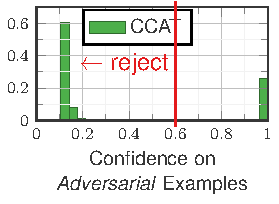
\includegraphics[height=4.25cm]{fig/histograms/succ_ours10_annotated}
		\end{minipage}
		\hfill
	\end{frame}

	\begin{frame}[t]{\bfseries \circled{1} Transition to Low Confidence}
		\Large
		
		\vspace*{0.25cm}
		\hspace*{0.05cm}
		\begin{minipage}{\textwidth}
			\begin{enumerate}
				\item Compute high-confidence adversarial examples:
				\vspace*{-0.25cm}
				\begin{align}
					\tilde{\delta} = \max_{\|\delta\|_\infty \leq \epsilon} \max_{\color{MPIIred}k\neq y}f_k(x + \delta;w)\notag
				\end{align}
				\begin{tikzpicture}[overlay]
				\node[MPIIblue] (text2) at (9, 0.5) {confidence of class $k$};
				\draw[arrow,MPIIblue] (text2)[out=180,in=290] to (6.2,0.9);
				\end{tikzpicture}
				\vspace*{-0.5cm}
				\item Impose target distribution via cross-entropy loss:
				\vspace*{-0.25cm}
				\begin{align}
					\tilde{y} = \lambda \,\,\text{one\_hot}(y) + (1-\lambda) \nicefrac{1}{K}\notag
				\end{align}
			\end{enumerate}
		\end{minipage}
	
		\centering
		%\vspace*{-0.15cm}
		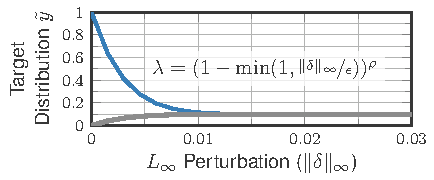
\includegraphics[height=3.5cm]{fig/transition/confidences_annotated}
	\end{frame}

	\begin{frame}[t]{\bfseries \circled{1} Transition to Low Confidence}
		\Large
		
		\vspace*{0.25cm}
		\hspace*{0.05cm}
		\begin{minipage}{\textwidth}
			\begin{enumerate}
				\item Compute high-confidence adversarial examples:
				\vspace*{-0.25cm}
				\begin{align}
				\tilde{\delta} = \max_{\|\delta\|_\infty \leq \epsilon} \max_{\color{MPIIred}k\neq y}f_k(x + \delta;w)\notag
				\end{align}
				\begin{tikzpicture}[overlay]
				\node[MPIIblue] (text2) at (9, 0.5) {confidence of class $k$};
				\draw[arrow,MPIIblue] (text2)[out=180,in=290] to (6.2,0.9);
				\end{tikzpicture}
				\vspace*{-0.5cm}
				\item Impose target distribution via cross-entropy loss:
				\vspace*{-0.25cm}
				\begin{align}
				\tilde{y} = \lambda \,\,\text{one\_hot}(y) + (1-\lambda) \nicefrac{1}{K}\notag
				\end{align}
			\end{enumerate}
		\end{minipage}
		
		\centering
		%\vspace*{-0.15cm}
		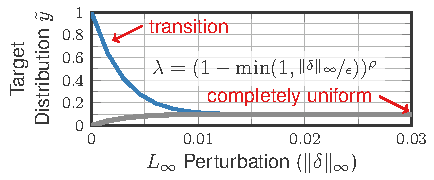
\includegraphics[height=3.5cm]{fig/transition/confidences_annotated2}
	\end{frame}

	\begin{frame}[t]{\bfseries \circled{2} Robustness by Confidence Thresholding}
		\Large 
		
		\begin{minipage}[t]{0.73\textwidth}
			\vspace*{0px}
			\hfill
			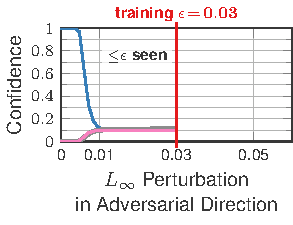
\includegraphics[width=8.5cm]{fig/introduction/ours10_1_adversarial_seen}
		\end{minipage}
		\hfill
		\begin{minipage}[t]{0.25\textwidth}
			\vspace*{20px}
			
			\begin{tcolorbox}[
				left=0pt,
				right=0pt,
				top=0pt,
				bottom=0pt,
				colback=gray!12!white,
				colframe=gray!12!white,
				width=1\textwidth, 
				enlarge left by=0mm,
				boxsep=5pt,
				arc=0pt,outer arc=0pt,
				%coltitle=black,
				%title=Training,
				boxrule=1pt,
				]
				\large\color{MPIIblack}
				SVHN:\\
				\textcolor{colorbrewer2}{{\rule[4pt]{10pt}{2pt} Correct}}\\ \textcolor{colorbrewer8}{{\rule[4pt]{10pt}{2pt} Adversarial}}
			\end{tcolorbox}
		\end{minipage}
	\end{frame}

	\begin{frame}[t]{\bfseries \circled{2} Robustness by Confidence Thresholding}
		\Large 
		
		\begin{minipage}[t]{0.73\textwidth}
			\vspace*{0px}
			\hfill
			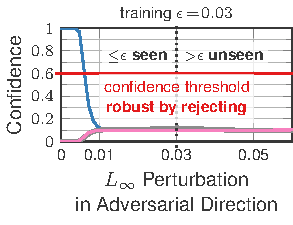
\includegraphics[width=8.5cm]{fig/introduction/ours10_1_adversarial_unseen_annotated}
		\end{minipage}
		\hfill
		\begin{minipage}[t]{0.25\textwidth}
			\vspace*{20px}
			
			\begin{tcolorbox}[
				left=0pt,
				right=0pt,
				top=0pt,
				bottom=0pt,
				colback=gray!12!white,
				colframe=gray!12!white,
				width=1\textwidth, 
				enlarge left by=0mm,
				boxsep=5pt,
				arc=0pt,outer arc=0pt,
				%coltitle=black,
				%title=Training,
				boxrule=1pt,
				]
				\large\color{MPIIblack}
				SVHN:\\
				\textcolor{colorbrewer2}{{\rule[4pt]{10pt}{2pt} Correct}}\\ \textcolor{colorbrewer8}{{\rule[4pt]{10pt}{2pt} Adversarial}}
			\end{tcolorbox}
		\end{minipage}
	\end{frame}
	
	\begin{frame}[t]{\bfseries \circled{2} Robustness by Confidence Thresholding}
		\Large 
		
		\vspace*{0.475cm}
		\begin{minipage}[t]{0.73\textwidth}
			\vspace*{0px}
			\hfill
			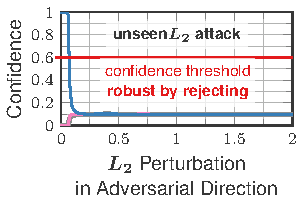
\includegraphics[width=8.91cm]{fig/introduction/ours10_3_l2_adversarial_annotated}
		\end{minipage}
		\hfill
		\begin{minipage}[t]{0.25\textwidth}
			\vspace*{6.5px}
			
			\begin{tcolorbox}[
				left=0pt,
				right=0pt,
				top=0pt,
				bottom=0pt,
				colback=gray!12!white,
				colframe=gray!12!white,
				width=1\textwidth, 
				enlarge left by=0mm,
				boxsep=5pt,
				arc=0pt,outer arc=0pt,
				%coltitle=black,
				%title=Training,
				boxrule=1pt,
				]
				\large\color{MPIIblack}
				SVHN:\\
				\textcolor{colorbrewer2}{{\rule[4pt]{10pt}{2pt} Correct}}\\ \textcolor{colorbrewer8}{{\rule[4pt]{10pt}{2pt} Adversarial}}
			\end{tcolorbox}
		\end{minipage}
	\end{frame}

    \begin{frame}[t]{\bfseries \circled{2} Meaningful Extrapolation of Confidence}
    	\Large 
    	
	    \vspace*{-0.25cm}    
	    \begin{tcolorbox}[
	    	enhanced,
	    	boxsep=0pt,
	    	left=5pt,
	    	right=5pt,
	    	top=0pt,
	    	toptitle=4pt,
	    	bottomtitle=2pt,
	    	bottom=0pt,
	    	colback=white,
	    	colframe=white,
	    	width=1\textwidth, 
	    	enlarge left by=0mm,
	    	arc=0pt,outer arc=0pt,
	    	%coltitle=black,
	    	%title=Training,
	    	boxrule=1pt,
	    	title=Adversarial training:,
	    	coltitle=MPIIblack,
	    	colbacktitle=white,
	    	titlerule style=white,
	    	]
	    	\vspace*{-2px}
	    	\centering
	    	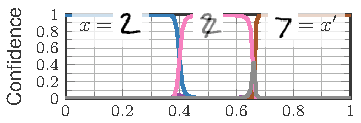
\includegraphics[width=8cm]{fig/interpolation/advtrain_0_interpolation}
	    \end{tcolorbox}
	    \vspace*{-4px}
	    
	    \begin{tcolorbox}[
	    	enhanced,
	    	boxsep=0pt,
	    	left=5pt,
	    	right=5pt,
	    	top=0pt,
	    	toptitle=4pt,
	    	bottomtitle=2pt,
	    	bottom=0pt,
	    	colback=white,%gray!12!white,
	    	colframe=gray!12!white,
	    	width=1\textwidth, 
	    	enlarge left by=0mm,
	    	arc=0pt,outer arc=0pt,
	    	%coltitle=black,
	    	%title=Training,
	    	boxrule=1pt,
	    	title=Confidence-calibrated adversarial training:,
	    	coltitle=MPIIblack,
	    	colbacktitle=gray!12!white,
	    	titlerule style=white,%gray!25!white,
	    	collower=MPIIblack,
	    	]
	    	\vspace*{-2px}
	    	\centering
	    	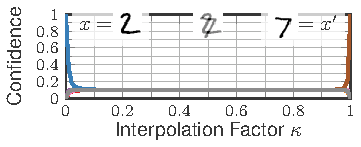
\includegraphics[width=8cm]{fig/interpolation/ours10_0_interpolation}
	    \end{tcolorbox}
    \end{frame}

	\begin{frame}[t]{\bfseries Summary: Generalizable Robustness}
		\Large
		
		Confidence-calibrated adversarial training:
		\vskip 0.1cm
		
		\circled{1} Transition: low confidence on adversarial examples.
		\vskip 0.25em
		
		\circled{2} {\color{MPIIred}Reject} low-confidence (adversarial) examples.
		
		\vspace*{-0.75cm}
		\begin{center}	
			%\vspace*{-4px}
			\begin{minipage}[t]{0.4\textwidth}
				\vspace*{0px}
				\hfill
				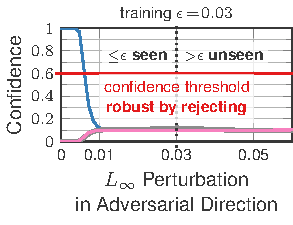
\includegraphics[width=4.75cm]{fig/introduction/ours10_1_adversarial_unseen_annotated}
			\end{minipage}
			\begin{minipage}[t]{0.4\textwidth}
				\vspace*{6px}
				\hfill
				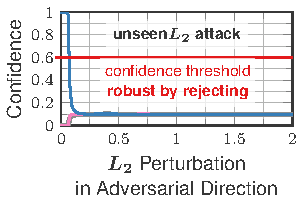
\includegraphics[width=4.9cm]{fig/introduction/ours10_3_l2_adversarial_annotated}
			\end{minipage}
%			\begin{minipage}[t]{0.3\textwidth}
%				\vspace*{9px}
%				\centering
%				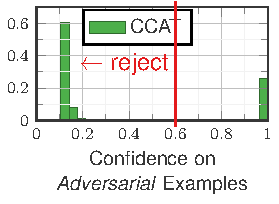
\includegraphics[width=3.5cm]{fig/histograms/succ_ours10_annotated}
%				\hfill
%			\end{minipage}
		\end{center}
		\vspace*{-0.5cm}
		\begin{itemize}
			%\item Low-confidence on adversarial examples \emph{and beyond}.
			\item {\bfseries Robustness to previously \emph{unseen} perturbations.}
		\end{itemize}
	\end{frame}

	\begin{frame}[t]{\bfseries ``Standard'' Robust Test Error \RTE}
		\Large
		
		= error on test examples that are ``attacked''.
		
		\vspace*{0.132cm}
		\begin{center}
			\begin{minipage}[t]{0.475\textwidth}
				\vspace*{0px}
				\centering
				Adversarial Training (AT):
				
				%$539$ of $1\text{k}$ adversarial examples successful
				
				57.3\% \RTE
				\vskip 0.5em
				
				\vphantom{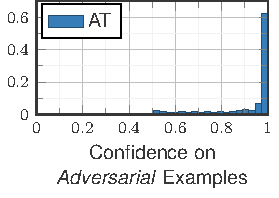
\includegraphics[width=5.75cm]{fig/histograms/succ_advtrain}\begin{tikzpicture}[overlay,fill=MPIIwhite,opacity=0.75]\node at(-2.5,2.5){Total: 539/1000};\end{tikzpicture}}
			\end{minipage}
			\hspace*{0.25cm}
			\begin{minipage}[t]{0.475\textwidth}
				\vspace*{0px}
				\centering
				Ours (CCAT):
				
				%$949$ of $1\text{k}$ adversarial examples successful
				
				97.8\% \RTE
				\vskip 0.5em
				
				\vphantom{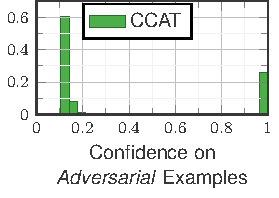
\includegraphics[width=5.75cm]{fig/histograms/succ_ours10}\begin{tikzpicture}[overlay,fill=MPIIwhite,opacity=0.75]\node at(-2.5,2.5){Total: 949/1000};\end{tikzpicture}}
			\end{minipage}
		\end{center}
	\end{frame}

	\begin{frame}[t]{\bfseries ``Standard'' Robust Test Error \RTE}
		\Large
		
		= error on test examples that are ``attacked''.
		
		\vspace*{0.132cm}
		\begin{center}
			\begin{minipage}[t]{0.475\textwidth}
				\vspace*{0px}
				\centering
				Adversarial Training (AT):
				
				%$539$ of $1\text{k}$ adversarial examples successful
				
				57.3\% \RTE
				\vskip 0.5em
				
				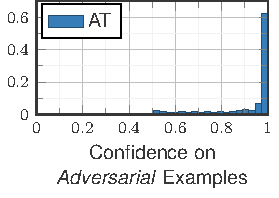
\includegraphics[width=5.75cm]{fig/histograms/succ_advtrain}\begin{tikzpicture}[overlay,fill=MPIIwhite,opacity=0.75]\node at(-2.5,2.5){Total: 539/1000};\end{tikzpicture}
			\end{minipage}
			\hspace*{0.25cm}
			\begin{minipage}[t]{0.475\textwidth}
				\vspace*{0px}
				\centering
				Ours (CCAT):
				
				%$949$ of $1\text{k}$ adversarial examples successful
				
				97.8\% \RTE
				\vskip 0.5em
				
				\includegraphics[width=5.75cm]{fig/histograms/succ_ours10}\begin{tikzpicture}[overlay,fill=MPIIwhite,opacity=0.75]\node at(-2.5,2.5){Total: 949/1000};\end{tikzpicture}
				%\includegraphics[width=5.75cm]{fig/histograms/succ_ours10_annotated}
			\end{minipage}
		\end{center}
	\end{frame}

	\begin{frame}[t]{\bfseries \textit{Confidence-Thresholded} \RTE}
		\Large
		
		= {\color{MPIIgray!40!MPIIblack}error on test examples that are ``attacked''}\\\hspace*{12px}and \emph{\textbf{pass} confidence thresholding}.
		
		\begin{center}
			\begin{minipage}{0.475\textwidth}
				\centering
				Adversarial Training (AT):
				
				%$539$ of $1\text{k}$ adversarial examples successful
				
				\textbf{56\%} ({\color{MPIIred} $-$1.3\%}) % 57.3\% \RTE
				\vskip 0.5em
				
				\includegraphics[width=5.75cm]{fig/histograms/succ_advtrain_annotated}
			\end{minipage}
			\hspace*{0.25cm}
			\begin{minipage}{0.475\textwidth}
				\centering
				Ours (CCAT):
				
				%$949$ of $1\text{k}$ adversarial examples successful
				
				\textbf{39.1\%}  ({\color{MPIIred} $-$58.7\%}) % 97.8\% \RTE
				\vskip 0.5em
				
				\includegraphics[width=5.75cm]{fig/histograms/succ_ours10_annotated}
			\end{minipage}
		\end{center}
	\end{frame}

	\begin{frame}[t]{\bfseries Determine Confidence Threshold}
		\Large
		
		\begin{itemize}
			\item Independent of adversarial examples.
			\item Avoid incorrectly rejecting (clean) test examples.
		\end{itemize}
		\vskip 0.3em
		
		{\bfseries Confidence threshold at 99\% true positive rate\hskip 2pxTPR:}
		
		\vspace*{-0.7cm}
		\begin{center}
			\begin{minipage}[t]{0.45\textwidth}
				\centering
				\vspace*{0px}
				
				\includegraphics[width=5.75cm]{fig/histograms/corr_ours10_annotated}
			\end{minipage}
			\hspace*{0.25cm}
			\begin{minipage}[t]{0.45\textwidth}
				\centering
				\vspace*{1px}
				
				\begin{tikzpicture}
					\node[opacity=0.5] at (0,0){\includegraphics[width=5.75cm]{fig/histograms/succ_ours10_bold}};
				\end{tikzpicture}
			\end{minipage}
		\end{center}
	\end{frame}

	\begin{frame}[t]{\bfseries Results}
		\Large
		
		Datasets: SVHN, CIFAR10, $1000$ test examples.
		\vskip 0.25cm
		
		\emph{Per-example}, worst-case (thresholded) \RTE across:
		\begin{center}
			\large 
			\begin{tabular}{| l | c | c |}
				\hline
				Attack & Iterations & Restarts\\\hline\hline
				PGD & 200-1000 & 10-50\\
				Query-Limited$^{\boldsymbol{\dagger}}$ & 1000 & 11\\ % \cite{IlyasICML2018b}
				Simple$^{\boldsymbol{\dagger}}$ & 1000 & 10\\ % \citep{NarodytskaCVPRWORK2017}
				Square$^{\boldsymbol{\dagger}}$ & 5000 & 1\\ % \citep{AndriushchenkoARXIV2019}
				%Corner Search$^{\boldsymbol{\dagger}}$ ($L_0$) & 200 & 1\\ % \citep{CroceARXIV2019}
				Geometry$^{\boldsymbol{\dagger}}$ & 1000 & 1\\ % \cite{KhouryARXIV2018}
				Random$^{\boldsymbol{\dagger}}$ & -- & 5000\\
				\hline
				\multicolumn{3}{l}{\footnotesize ($\boldsymbol{\dagger}$ Black-box attacks.)}
			\end{tabular}
		\end{center}
		\vspace*{-0.25cm}
		\begin{itemize}
			\item Attacks adapted to maximize confidence.
		\end{itemize}
	\end{frame}

	\begin{frame}{\bfseries SVHN: Generalization to Unseen Attacks}
		\Large 
		\begin{table}
			\centering
			% 2020-01-28 18:48:24.475299
\begin{tabularx}{1\textwidth}{|X|@{ }c@{ }|@{ }c@{ }|@{ }c@{ }|@{ }c@{ }|@{ }c@{ }|}
\hline
\multicolumn{6}{|c|}{\textbf{SVHN:} \textbf{\RTE} $\downarrow$ in \% at $99\%$TPR}\\
\hline
& \multicolumn{1}{@{}c@{}|@{ }}{\begin{tabular}{@{}c@{}}$L_\infty$\\$\epsilon = 0.03$\end{tabular}}
& %\multicolumn{1}{@{}c@{}|@{ }}{\begin{tabular}{@{}c@{}}$L_\infty$\\$\epsilon = 0.06$\end{tabular}}
& %\multicolumn{1}{@{}c@{}|@{ }}{\begin{tabular}{@{}c@{}}$L_2$\\$\epsilon = 2$\end{tabular}}
& %\multicolumn{1}{@{}c@{}|@{ }}{\begin{tabular}{@{}c@{}}$L_1$\\$\epsilon = 24$\end{tabular}}
& %\multicolumn{1}{c|}{\begin{tabular}{@{}c@{}}$L_0$\\$\epsilon = 10$\end{tabular}}
%& \multicolumn{1}{c|}{\begin{tabular}{@{}c@{}}adv.\\frames\end{tabular}}
\\\hline
& \multicolumn{1}{@{}c@{}|@{ }}{\textcolor{colorbrewer3}{seen}}
& \multicolumn{1}{@{}c@{}|@{ }}{\textcolor{white}{\bfseries unseen}}
& \multicolumn{1}{@{}c@{}|@{ }}{\textcolor{white}{\bfseries unseen}}
& \multicolumn{1}{@{}c@{}|@{ }}{\textcolor{white}{\bfseries unseen}}
& \multicolumn{1}{c|}{\textcolor{white}{\bfseries unseen}}
%& \multicolumn{1}{c|}{\textcolor{colorbrewer1}{\bfseries unseen}}
\\\hline
%& \RTE$\downarrow$
%& %\RTE$\downarrow$
%& %\RTE$\downarrow$
%& %\RTE$\downarrow$
%& %\RTE$\downarrow$
%& \RTE$\downarrow$
%\\\hline
\hline
AT & 56.0 % fpr@99, rte@99
& %88.4 % fpr@99, rte@99
& %99.4 % fpr@99, rte@99
& %99.5 % fpr@99, rte@99
& %73.6 % fpr@99, rte@99
%& 33.6 % fpr@99, rte@99
\\
CCAT & \bfseries 39.1 % fpr@99, rte@99
& %\bfseries 53.1 % fpr@99, rte@99
& %\bfseries 29.0 % fpr@99, rte@99
& %\bfseries 31.7 % fpr@99, rte@99
& %\bfseries 3.5 % fpr@99, rte@99
%& \bfseries 3.7 % fpr@99, rte@99
\\\hline
\multicolumn{6}{l}{\large (Lower \RTE $\downarrow$ means ``better'' robustness.)}
\end{tabularx}

		\end{table}
	\end{frame}

	\begin{frame}{\bfseries SVHN: Generalization to Unseen Attacks}
		\Large 
		\begin{table}
			\centering
			% 2020-01-28 18:48:24.475299
\begin{tabularx}{1\textwidth}{|X|@{ }c@{ }|@{ }c@{ }|@{ }c@{ }|@{ }c@{ }|@{ }c@{ }|}
\hline
\multicolumn{6}{|c|}{\textbf{SVHN:} \textbf{\RTE} $\downarrow$ in \% at $99\%$TPR}\\
\hline
& \multicolumn{1}{@{}c@{}|@{ }}{\begin{tabular}{@{}c@{}}$L_\infty$\\$\epsilon = 0.03$\end{tabular}}
& \multicolumn{1}{@{}c@{}|@{ }}{\begin{tabular}{@{}c@{}}$L_\infty$\\$\epsilon = 0.06$\end{tabular}}
& \multicolumn{1}{@{}c@{}|@{ }}{\begin{tabular}{@{}c@{}}$L_2$\\$\epsilon = 2$\end{tabular}}
& \multicolumn{1}{@{}c@{}|@{ }}{\begin{tabular}{@{}c@{}}$L_1$\\$\epsilon = 24$\end{tabular}}
& \multicolumn{1}{c|}{\begin{tabular}{@{}c@{}}$L_0$\\$\epsilon = 10$\end{tabular}}
%& \multicolumn{1}{c|}{\begin{tabular}{@{}c@{}}adv.\\frames\end{tabular}}
\\\hline
& \multicolumn{1}{@{}c@{}|@{ }}{\textcolor{colorbrewer3}{seen}}
& \multicolumn{1}{@{}c@{}|@{ }}{\textcolor{colorbrewer1}{\bfseries unseen}}
& \multicolumn{1}{@{}c@{}|@{ }}{\textcolor{colorbrewer1}{\bfseries unseen}}
& \multicolumn{1}{@{}c@{}|@{ }}{\textcolor{colorbrewer1}{\bfseries unseen}}
& \multicolumn{1}{c|}{\textcolor{colorbrewer1}{\bfseries unseen}}
%& \multicolumn{1}{c|}{\textcolor{colorbrewer1}{\bfseries unseen}}
\\\hline
%& \RTE$\downarrow$
%& \RTE$\downarrow$
%& \RTE$\downarrow$
%& \RTE$\downarrow$
%& \RTE$\downarrow$
%& \RTE$\downarrow$
%\\\hline
\hline
AT & 56.0 % fpr@99, rte@99
& %88.4 % fpr@99, rte@99
& %99.4 % fpr@99, rte@99
& %99.5 % fpr@99, rte@99
& %73.6 % fpr@99, rte@99
%& 33.6 % fpr@99, rte@99
\\
CCAT & \bfseries 39.1 % fpr@99, rte@99
& %\bfseries 53.1 % fpr@99, rte@99
& %\bfseries 29.0 % fpr@99, rte@99
& %\bfseries 31.7 % fpr@99, rte@99
& %\bfseries 3.5 % fpr@99, rte@99
%& \bfseries 3.7 % fpr@99, rte@99
\\\hline
\multicolumn{6}{l}{\large (Lower \RTE $\downarrow$ means ``better'' robustness.)}
\end{tabularx}

		\end{table}
	\end{frame}

	\begin{frame}{\bfseries SVHN: Generalization to Unseen Attacks}
		\Large 
		\begin{table}
			\centering
			% 2020-01-28 18:48:24.475299
\begin{tabularx}{1\textwidth}{|X|@{ }c@{ }|@{ }c@{ }|@{ }c@{ }|@{ }c@{ }|@{ }c@{ }|}
\hline
\multicolumn{6}{|c|}{\textbf{SVHN:} \textbf{\RTE} $\downarrow$ in \% at $99\%$TPR}\\
\hline
& \multicolumn{1}{@{}c@{}|@{ }}{\begin{tabular}{@{}c@{}}$L_\infty$\\$\epsilon = 0.03$\end{tabular}}
& \multicolumn{1}{@{}c@{}|@{ }}{\begin{tabular}{@{}c@{}}$L_\infty$\\$\epsilon = 0.06$\end{tabular}}
& \multicolumn{1}{@{}c@{}|@{ }}{\begin{tabular}{@{}c@{}}$L_2$\\$\epsilon = 2$\end{tabular}}
& \multicolumn{1}{@{}c@{}|@{ }}{\begin{tabular}{@{}c@{}}$L_1$\\$\epsilon = 24$\end{tabular}}
& \multicolumn{1}{c|}{\begin{tabular}{@{}c@{}}$L_0$\\$\epsilon = 10$\end{tabular}}
%& \multicolumn{1}{c|}{\begin{tabular}{@{}c@{}}adv.\\frames\end{tabular}}
\\\hline
& \multicolumn{1}{@{}c@{}|@{ }}{\textcolor{colorbrewer3}{seen}}
& \multicolumn{1}{@{}c@{}|@{ }}{\textcolor{colorbrewer1}{\bfseries unseen}}
& \multicolumn{1}{@{}c@{}|@{ }}{\textcolor{colorbrewer1}{\bfseries unseen}}
& \multicolumn{1}{@{}c@{}|@{ }}{\textcolor{colorbrewer1}{\bfseries unseen}}
& \multicolumn{1}{c|}{\textcolor{colorbrewer1}{\bfseries unseen}}
%& \multicolumn{1}{c|}{\textcolor{colorbrewer1}{\bfseries unseen}}
\\\hline
%& \RTE$\downarrow$
%& \RTE$\downarrow$
%& \RTE$\downarrow$
%& \RTE$\downarrow$
%& \RTE$\downarrow$
%& \RTE$\downarrow$
%\\\hline
\hline
AT & 56.0 % fpr@99, rte@99
& 88.4 % fpr@99, rte@99
& 99.4 % fpr@99, rte@99
& 99.5 % fpr@99, rte@99
& 73.6 % fpr@99, rte@99
%& 33.6 % fpr@99, rte@99
\\
CCAT & \bfseries 39.1 % fpr@99, rte@99
& \bfseries 53.1 % fpr@99, rte@99
& \bfseries 29.0 % fpr@99, rte@99
& \bfseries 31.7 % fpr@99, rte@99
& \bfseries 3.5 % fpr@99, rte@99
%& \bfseries 3.7 % fpr@99, rte@99
\\\hline
\multicolumn{6}{l}{\large (Lower \RTE $\downarrow$ means ``better'' robustness.)}
\end{tabularx}

		\end{table}
	\end{frame}

	\begin{frame}{\bfseries Cifar10: Generalization to Unseen Attacks}
		\Large 
		\begin{table}
			\centering
			% 2020-01-27 19:07:45.500359
\begin{tabularx}{1\textwidth}{|X|@{ }c@{ }|@{ }c@{ }|@{ }c@{ }|@{ }c@{ }|@{ }c@{ }|}
\hline
\multicolumn{6}{|c|}{\textbf{CIFAR10:} \textbf{\RTE} $\downarrow$ in \% at $99\%$TPR}\\
\hline
& \multicolumn{1}{@{}c@{}|@{ }}{\begin{tabular}{@{}c@{}}$L_\infty$\\$\epsilon = 0.03$\end{tabular}}
& \multicolumn{1}{@{}c@{}|@{ }}{\begin{tabular}{@{}c@{}}$L_\infty$\\$\epsilon = 0.06$\end{tabular}}
& \multicolumn{1}{@{}c@{}|@{ }}{\begin{tabular}{@{}c@{}}$L_2$\\$\epsilon = 2$\end{tabular}}
& \multicolumn{1}{@{}c@{}|@{ }}{\begin{tabular}{@{}c@{}}$L_1$\\$\epsilon = 24$\end{tabular}}
& \multicolumn{1}{c|}{\begin{tabular}{@{}c@{}}$L_0$\\$\epsilon = 10$\end{tabular}}
%& \multicolumn{1}{c|}{\begin{tabular}{@{}c@{}}adv.\\frames\end{tabular}}
\\\hline
& \multicolumn{1}{@{}c@{}|@{ }}{\textcolor{colorbrewer3}{seen}}
& \multicolumn{1}{@{}c@{}|@{ }}{\textcolor{colorbrewer1}{\bfseries unseen}}
& \multicolumn{1}{@{}c@{}|@{ }}{\textcolor{colorbrewer1}{\bfseries unseen}}
& \multicolumn{1}{@{}c@{}|@{ }}{\textcolor{colorbrewer1}{\bfseries unseen}}
& \multicolumn{1}{c|}{\textcolor{colorbrewer1}{\bfseries unseen}}
%& \multicolumn{1}{c|}{\textcolor{colorbrewer1}{\bfseries unseen}}
\\\hline
%& \RTE$\downarrow$
%& \RTE$\downarrow$
%& \RTE$\downarrow$
%& \RTE$\downarrow$
%& \RTE$\downarrow$
%& \RTE$\downarrow$
%\\\hline
\hline
AT & \bfseries 62.7 % fpr@98, rte@98
& 93.7 % fpr@98, rte@98
& 98.4 % fpr@98, rte@98
& 98.4 % fpr@98, rte@98
& 72.4 % fpr@98, rte@98
%& 78.7 % fpr@98, rte@98
\\
CCAT & 67.9 % fpr@98, rte@98
& 92.0 % fpr@98, rte@98
& \bfseries 51.8 % fpr@98, rte@98
& \bfseries 58.5 % fpr@98, rte@98
& \bfseries 20.3 % fpr@98, rte@98
%& \bfseries 65.1 % fpr@98, rte@98
\\
\hline
\multicolumn{6}{l}{\large (Lower \RTE $\downarrow$ means ``better'' robustness.)}
\end{tabularx}

		\end{table}
	\end{frame}

	\begin{frame}{\bfseries ``Unconventional'' Attacks}
		\Large
		
		\vspace*{-0.5cm} 
		\begin{table}
			\centering
			% 2020-01-27 19:07:45.500359
\begin{tabularx}{1\textwidth}{|X|@{ }c@{ }|@{ }c@{ }|@{ }c@{ }|}
	\hline
	\multicolumn{4}{|c|}{\textbf{CIFAR10:} \RTE, FPR and CErr at $99\%$TPR}\\
	\hline
	& \multicolumn{1}{@{ }c@{ }|@{ }}{\begin{tabular}{@{}c@{}}adv.\\frames\end{tabular}}
	& \multicolumn{1}{@{ }c@{ }|@{ }}{\begin{tabular}{@{}c@{}}distal\end{tabular}}
	& \multicolumn{1}{@{ }c@{ }|}{\begin{tabular}{@{}c@{}}corrupted\end{tabular}}
	\\\hline
	& \multicolumn{1}{@{ }c@{ }|@{ }}{\textcolor{colorbrewer1}{\bfseries unseen}}
	& \multicolumn{1}{@{ }c@{ }|@{ }}{\textcolor{colorbrewer1}{\bfseries unseen}}
	& \multicolumn{1}{@{ }c@{ }|}{\textcolor{colorbrewer1}{\bfseries unseen}}
	\\\hline
	& \RTE$\downarrow$
	& FPR$\downarrow$
	& CErr$\downarrow$
	%& \RTE$\downarrow$
	\\\hline\hline
	Normal & 96.6
	& 83.3
	& 12.3
	\\
	AT & 78.7
	& 75.0
	& 16.2
	\\
	CCAT & \bfseries 65.1
	& \bfseries 0
	& \bfseries 8.5
	\\
	\hline
	\multicolumn{4}{l}{\large (FPR: false positive rate, fraction of non-rejected adv. examples.)}\\
	\multicolumn{4}{l}{\large (CErr: test error on corrupted examples after thresholding.)}\\
\end{tabularx}

		\end{table}
	\end{frame}

	\begin{frame}{\bfseries Improved Accuracy}
		\Large
		
		\vspace*{-1.25cm}
		\begin{table}
			\centering
			\begin{minipage}[t]{0.5\textwidth}
				\vspace*{0px}
				
				\begin{tabular}{|@{ }c@{ }|@{ }c@{ }|}
    \hline
    \multicolumn{2}{|c|}{\textbf{CIFAR10:}}\\
    \multicolumn{2}{|c|}{Err $\downarrow$ in \%}\\
    \hline
    \hline
    \begin{tabular}{@{}c@{}}no\\reject\end{tabular} &
    \begin{tabular}{@{}c@{}}$99\%$\\TPR\end{tabular}\\
    \hline
    \hline
    %\begin{tabular}{@{}c@{}}\TE\\in \%\end{tabular} &
    %\begin{tabular}{@{}c@{}}\TE\\in \%\end{tabular}\\
    %\hline
    \bfseries 8.3 & 7.4\\
    16.6 & 15.5\\
    10.1 & \bfseries 6.7\\
    \hline
\end{tabular}
			\end{minipage}
			\begin{minipage}[t]{0.29\textwidth}
				\vspace*{0px}
				 
				\begin{tabular}{|@{ }c@{ }|@{ }c@{ }|}
    \hline
    \multicolumn{2}{|c|}{\textbf{CIFAR10:}}\\
    \multicolumn{2}{|c|}{Err $\downarrow$ in \%}\\
    \hline
    \hline
    \begin{tabular}{@{}c@{}}no\\reject\end{tabular} &
    \begin{tabular}{@{}c@{}}$99\%$\\TPR\end{tabular}\\
    \hline
    \hline
    %\begin{tabular}{@{}c@{}}\TE\\in \%\end{tabular} &
    %\begin{tabular}{@{}c@{}}\TE\\in \%\end{tabular}\\
    %\hline
    \bfseries 8.3 & 7.4\\
    16.6 & 15.5\\
    10.1 & \bfseries 6.7\\
    \hline
\end{tabular}
			\end{minipage}
			\vspace*{2px}
			
			\large
			\raggedright
			\hspace*{1.2cm}(Err: test error before and after thresholding.)
		\end{table}
	\end{frame}

	\begin{frame}[t]{\bfseries Confidence-Calibrated Adversarial Training}
		\Large
		
		\vspace*{-0.15cm}
		%Confidence-calibrated adversarial training\\
		Low-confidence on adversarial examples and \emph{beyond}.
		\begin{itemize}
			\item Robustness generalizes to unseen attacks.
			\item Accuracy improves.
		\end{itemize}
	
		\vspace*{-0.3cm}
		\begin{center}
			\begin{minipage}[t]{0.475\textwidth}
				\begin{tcolorbox}[
					enhanced,
					boxsep=0pt,
					left=5pt,
					right=5pt,
					top=0pt,
					toptitle=4pt,
					bottomtitle=4pt,
					bottom=0pt,
					colback=white,
					colframe=gray!25!white,
					width=1\textwidth, 
					enlarge left by=0mm,
					arc=0pt,outer arc=0pt,
					%coltitle=black,
					%title=Training,
					boxrule=1pt,
					title=\large Adversarial training:,
					coltitle=MPIIblack,
					colbacktitle=white,%gray!12!white,
					%titlerule style=gray!25!white,
					collower=MPIIblack,
					]
				\includegraphics[width=5cm]{fig/introduction/advtrain_1_adversarial_unseen_narrow}
				\end{tcolorbox}
			\end{minipage}
			\begin{minipage}[t]{0.475\textwidth}
				\begin{tcolorbox}[
					enhanced,
					boxsep=0pt,
					left=5pt,
					right=5pt,
					top=0pt,
					toptitle=4pt,
					bottomtitle=4pt,
					bottom=0pt,
					colback=gray!12!white,
					colframe=gray!12!white,
					width=1\textwidth, 
					enlarge left by=0mm,
					arc=0pt,outer arc=0pt,
					%coltitle=black,
					%title=Training,
					boxrule=1pt,
					title=\large Ours\vphantom{g}:,
					coltitle=MPIIblack,
					colbacktitle=gray!12!white,
					titlerule style=white,%gray!25!white,
					collower=MPIIblack,
					]
				\includegraphics[width=5cm]{fig/introduction/ours10_1_adversarial_unseen_annotated_narrow}
				\end{tcolorbox}
			\end{minipage}
			\begin{minipage}[t]{0.9625\textwidth}
				\begin{tcolorbox}[
					enhanced,
					boxsep=3pt,
					left=0pt,
					right=0pt,
					top=0pt,
					toptitle=0pt,
					bottomtitle=0pt,
					bottom=0pt,
					colback=gray!12!white,
					colframe=gray!12!white,
					width=1\textwidth, 
					enlarge left by=0mm,
					arc=0pt,outer arc=0pt,
					%coltitle=black,
					%title=Training,
					boxrule=1pt,
					%title=\large Ours:,
					coltitle=MPIIblack,
					colbacktitle=gray!12!white,
					titlerule style=white,%gray!25!white,
					collower=MPIIblack,
					]
					\color{MPIIblack}
					Paper \& code: \href{http://davidstutz.de/ccat}{\texttt{davidstutz.de/ccat}}
				\end{tcolorbox}
			\end{minipage}
		\end{center}
	\end{frame}
\end{document}
